% Provide a two-screen representation of the flow (vertically-side by side) for either 2 of the
% 3 plots you have shown in Tasks 1 − 3. Provide a description of how combining these flow
% illsutrations will assist your understanding of the flow physics. Use screenshots and other
% illustrations to support your statement.

\section{}
\textit{Provide a two-screen representation of the flow (vertically-side by side) for either 2 of the 3 plots you have shown in Tasks 1 - 3. Provide a description of how combining these flow illustrations will assist your understanding of the flow physics. Use screenshots and other illustrations to support your statement.}

\subsection*{Solution}
\begin{figure}[h]
    \centering
    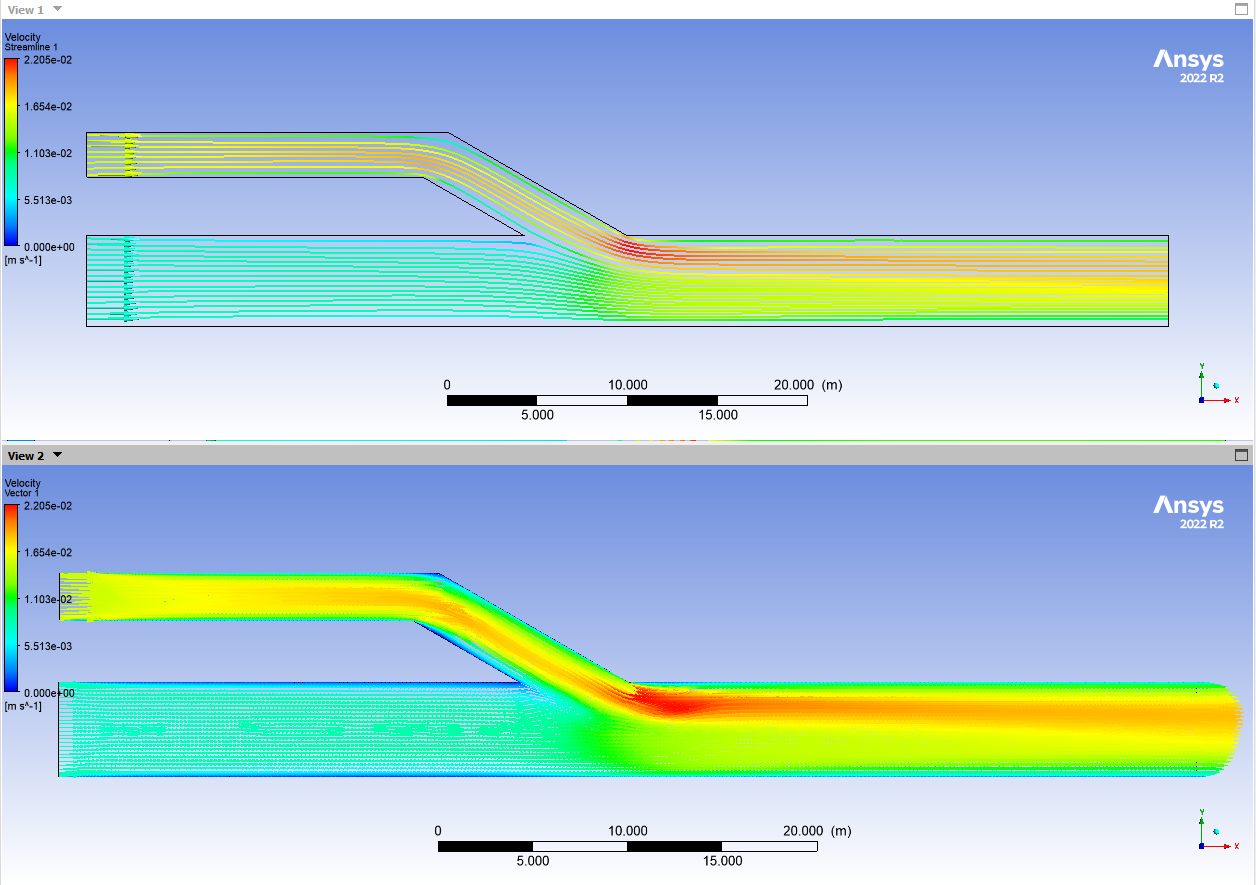
\includegraphics[width=0.8\textwidth]{Questions/Figures/velocity streamline and vector.png}
    \caption{Streamline and vector plot of the flow velocity}
    \label{fig:contour}
\end{figure}

The streamline plot follows the tangential direction of the flow, showing the path taken by a particular fluid particle. The vector plot shows the magnitude and direction of the flow at a particular point. 

The streamline plot is useful if we want to see the path taken by a particular fluid particle. The vector plot is useful if we want to see the magnitude and direction of the flow at a particular point or if we want to see the flow field as a whole.